% RenderLab - Project Report (JIIT, Dept. of CSE & IT)
% Format copied from the Klaro report template: A4, 11 pt text, 13 pt bold main headings,
% 12 pt bold sub-headings, 1.5 line spacing, margins L 3.5 cm / T 2.5 cm / R 1.25 cm / B 1.25 cm.
% Build: tectonic main.tex

\documentclass[11pt,a4paper,oneside]{report}

% ---------------------------------------------------------------- fill these in
\newcommand{\projecttitle}{RenderLab, a software-rasterizer graphics laboratory}
\newcommand{\coursename}{Geometric Algebra for Computer Graphics}
\newcommand{\coursecode}{22B12MA412}
\newcommand{\programme}{B. Tech. CSE}
\newcommand{\semester}{Semester VII}
\newcommand{\session}{2026 - 2027 (odd semester)}
\newcommand{\studentA}{Yasharth Singh} \newcommand{\enrolA}{9923103059}
\newcommand{\studentB}{Rakshit Suneja} \newcommand{\enrolB}{9923102028}
\newcommand{\coordinator}{Dr. Ajay Kumar Gupta}
\newcommand{\subdate}{November 2026}
% ------------------------------------------------------------------------------

\usepackage[a4paper,left=3.5cm,top=2.5cm,right=1.25cm,bottom=1.25cm,footskip=0.6cm]{geometry}
\usepackage[T1]{fontenc}
\usepackage{newtxtext,newtxmath}
\usepackage{setspace}
\onehalfspacing
\emergencystretch=2em
\usepackage{graphicx}
\usepackage{float}
\usepackage{booktabs,tabularx,array}
\usepackage{enumitem}
\setlist{nosep,leftmargin=1.5em}
\usepackage{xcolor}
\usepackage{url}
\usepackage{caption}
\captionsetup{font=small,labelfont=bf,skip=4pt}
\captionsetup[table]{position=top}
\usepackage{titlesec}
\usepackage{fancyhdr}
\usepackage{tocloft}
\usepackage{tikz}
\usetikzlibrary{arrows.meta,positioning,fit,calc,shapes.geometric,shapes.misc,shapes.symbols}
\usepackage{listings}
\lstdefinestyle{code}{basicstyle=\ttfamily\footnotesize,breaklines=true,frame=single,framerule=0.3pt,rulecolor=\color{black!40},backgroundcolor=\color{black!3},xleftmargin=0pt,aboveskip=2pt,belowskip=2pt,columns=fullflexible,keepspaces=true}
\usepackage[hidelinks]{hyperref}

% Headings: main 13 pt bold, sub 12 pt bold, sub-sub 11 pt bold.
\titleformat{\chapter}[block]{\fontsize{13}{16}\selectfont\bfseries\centering}{Chapter \thechapter:}{0.4em}{}
\titleformat{name=\chapter,numberless}[block]{\fontsize{13}{16}\selectfont\bfseries\centering}{}{0pt}{}
\titlespacing*{\chapter}{0pt}{0pt}{10pt}
\titleformat{\section}{\fontsize{12}{14}\selectfont\bfseries}{\thesection}{0.6em}{}
\titlespacing*{\section}{0pt}{8pt}{4pt}
\titleformat{\subsection}{\fontsize{11}{13}\selectfont\bfseries}{\thesubsection}{0.6em}{}
\titlespacing*{\subsection}{0pt}{6pt}{2pt}

% Page numbers at the bottom centre. The first page of a numbered chapter has none (\nonum after \chapter).
\pagestyle{fancy}
\fancyhf{}
\fancyfoot[C]{\thepage}
\renewcommand{\headrulewidth}{0pt}
\fancypagestyle{plain}{\fancyhf{}\fancyfoot[C]{\thepage}\renewcommand{\headrulewidth}{0pt}}
\newcommand{\nonum}{}% chapter first pages are numbered too (was \thispagestyle{empty})

% Table of contents: headings and next sub-headings only.
\setcounter{tocdepth}{1}
\setcounter{secnumdepth}{2}
\renewcommand{\contentsname}{Table of Contents}
\renewcommand{\cftchappresnum}{Chapter }
\renewcommand{\cftchapaftersnum}{:}
\setlength{\cftchapnumwidth}{5.6em}
\cftpagenumbersoff{chapter}
\renewcommand{\cftchapfont}{\bfseries}
\setlength{\cftbeforesecskip}{1pt}
\setlength{\cftbeforechapskip}{6pt}
\renewcommand{\cfttoctitlefont}{\hfill\fontsize{13}{16}\selectfont\bfseries}
\renewcommand{\cftaftertoctitle}{\hfill\hfill\par\noindent\hfill\textbf{Page No.}}
\renewcommand{\cftlottitlefont}{\hfill\fontsize{13}{16}\selectfont\bfseries}
\renewcommand{\cftafterlottitle}{\hfill\hfill\par\noindent\textbf{Table}\hspace{3.3em}\textbf{Title}\hfill\textbf{Page}}
\renewcommand{\cftloftitlefont}{\hfill\fontsize{13}{16}\selectfont\bfseries}
\renewcommand{\cftafterloftitle}{\hfill\hfill\par\noindent\textbf{Figure}\hspace{3em}\textbf{Title}\hfill\textbf{Page}}
\setlength{\cftbeforetoctitleskip}{0pt}
\setlength{\cftbeforelottitleskip}{0pt}
\setlength{\cftbeforeloftitleskip}{0pt}
\setlength{\cftaftertoctitleskip}{8pt}
\setlength{\cftafterlottitleskip}{8pt}
\setlength{\cftafterloftitleskip}{8pt}
\setlength{\cfttabnumwidth}{4.5em}
\setlength{\cftfignumwidth}{4.5em}
\setlength{\cfttabindent}{0pt}
\setlength{\cftfigindent}{0pt}

\newcolumntype{L}{>{\raggedright\arraybackslash}X}
% A table-of-contents line with its page number, as in the template (italic for the front matter).
\newcommand{\tocline}[3]{\par\noindent{#1#2}\cftdotfill{\cftdotsep}{#1#3}\par\vspace{2pt}}
\newcommand{\addtocline}[2]{\addtocontents{toc}{\protect\tocline{#1}{#2}{\thepage}}}

% A screenshot: the real file when it exists, otherwise a grey box with the expected file name.
\newcommand{\shot}[2]{\IfFileExists{figures/#1}{\includegraphics[width=#2]{figures/#1}}{%
  \fcolorbox{black!40}{black!8}{\parbox[c][3.2cm][c]{#2}{\centering\small MISSING SCREENSHOT:\\\texttt{\detokenize{#1}}}}}}

% Flowchart styles: light fills that print well in colour and in greyscale.
\colorlet{cStep}{blue!55!black}
\colorlet{cAI}{orange!80!black}
\colorlet{cData}{teal!70!black}
\colorlet{cUser}{violet!70!black}
\tikzset{
  base/.style={draw, thick, rounded corners=4pt, align=center, font=\small, inner sep=5pt},
  proc/.style={base, draw=cStep, fill=cStep!7},
  ai/.style={base, draw=cAI, fill=cAI!10},
  data/.style={base, draw=cData, fill=cData!8},
  user/.style={base, draw=cUser, fill=cUser!8},
  term/.style={base, draw=cUser, fill=cUser!8, rounded rectangle},
  decide/.style={draw=cAI, thick, fill=yellow!15, diamond, aspect=2.2, align=center, font=\small, inner sep=1pt},
  sub/.style={font=\scriptsize\color{black!70}},
  arr/.style={-{Stealth[length=2.4mm]}, thick, draw=black!70},
  lbl/.style={font=\scriptsize\itshape, align=center, text=black!75},
  zone/.style={draw=black!45, dashed, rounded corners=6pt, inner sep=7pt},
  ztitle/.style={font=\scriptsize\bfseries, text=black!65},
}
% A two-line step: bold title, small plain description.
\newcommand{\st}[2]{\textbf{#1}\\[-1pt]{\scriptsize #2}}


\newcommand{\twoshot}[4]{\begin{figure}[H]\centering\shot{#1}{0.49\linewidth}\hfill\shot{#2}{0.49\linewidth}\caption{#3}\label{#4}\end{figure}}

\begin{document}

% ============================================================ COVER PAGE
\pagenumbering{gobble}
\begin{titlepage}
\centering
{\fontsize{18}{22}\selectfont\bfseries Jaypee Institute of Information Technology, Noida\par}
\vspace{10pt}
{\fontsize{14}{17}\selectfont DEPARTMENT OF COMPUTER SCIENCE \& ENGINEERING AND INFORMATION TECHNOLOGY\par}
\vspace{1.2cm}

\includegraphics[height=5.2cm]{figures/jiit_logo.png}
\par\vspace{1.4cm}
{\fontsize{16}{20}\selectfont\textbf{Project Title:} \projecttitle\par}
\vspace{1.2cm}
{\fontsize{12}{15}\selectfont\raggedright
\hspace*{2in}\begin{tabular}{@{}p{3.2cm}l@{}}
\textbf{Enrol. No.} & \textbf{Name of Student}\\[6pt]
\enrolA & \studentA\\[4pt]
\enrolB & \studentB\\
\end{tabular}\par}
\vspace{1.4cm}
{\fontsize{12}{15}\selectfont
Course Name: \coursename\\[6pt]
Course Code: \coursecode\\[6pt]
Program: \programme\\[6pt]
\semester\\[6pt]
\textbf{\session}\par}
\vfill
\end{titlepage}

% ============================================================ ACKNOWLEDGEMENT
\pagenumbering{roman}
\chapter*{ACKNOWLEDGEMENT}
\addtocline{\itshape}{Acknowledgement}
We would like to place on record our sincere thanks to \coordinator, course coordinator for
Geometric Algebra for Computer Graphics (\coursecode), Jaypee Institute of Information Technology,
Noida, for the course that gave this project its topics and for the guidance given while we worked on it.

We also thank our classmates for trying the labs and for their comments on how the screens could be made clearer.

% ============================================================ ABSTRACT
\chapter*{ABSTRACT}
\addtocline{\itshape}{Abstract}
RenderLab is a program that runs in a web browser and helps a student see how computer graphics works. Every picture on the screen is drawn by our own code. The code writes colours into an array of pixels and the browser shows that array. We did not use WebGL or any 3D library.

The project is made for the course Geometric Algebra for Computer Graphics. It has the four algorithms the course asks for: Bresenham line drawing, back-face culling, alpha compositing (the Porter--Duff ``over'' rule) and Visvalingam--Whyatt line simplification. Each one has its own lab. The lab shows the formulas, the numbers at each step, and a comparison with a simpler or wrong version. Other labs cover 2D and 3D transformations, determinants, quaternions against Euler angles, the outer product, the sine rule, line intersection, bases and handedness. As extras, there is a demo scene with a small scene editor, and a benchmark tab that times our code.

All 487 automated tests pass. We tried all 195 controls by hand and fixed two layout bugs. In the benchmark (15 timed runs after 5 warm-up runs), back-face culling removed 50.33\% of the 15,412 triangles of the demo scene and cut the time for one frame from 41.4 ms to 28.0 ms. The older DDA line method was faster than Bresenham in JavaScript (68 ms against 122.5 ms for 10,000 long lines). Visvalingam--Whyatt took 14.3 ms for 2,000 points, and its time grew roughly with the square of the number of points.

\vspace{6pt}
\noindent\textbf{Keywords:} software rasterizer, Bresenham, back-face culling, alpha compositing, Visvalingam--Whyatt, quaternion, outer product.


% ============================================================ TOC, LISTS
\cleardoublepage
\tableofcontents
\cleardoublepage
\addtocline{\itshape}{List of Tables}
\listoftables
\cleardoublepage
\addtocline{\itshape}{List of Figures}
\listoffigures

\cleardoublepage
\chapter*{List of Abbreviations}
\addtocline{\itshape}{List of Abbreviations}
\begin{tabular}{@{}p{2.6cm}l@{}}
CPU & Central Processing Unit\\
CSV & Comma-Separated Values (a plain table file)\\
DDA & Digital Differential Analyzer (a simple line-drawing method)\\
NDC & Normalized Device Coordinates (the cube $-1$ to $1$ the camera maps the scene into)\\
RDP & Ramer--Douglas--Peucker (a line simplification algorithm)\\
RGBA & Red, Green, Blue, Alpha\\
SIGGRAPH & Special Interest Group on Computer Graphics and Interactive Techniques\\
UI & User Interface\\
VW & Visvalingam--Whyatt (a line simplification algorithm)\\
\end{tabular}


% ============================================================ MAIN MATTER
\cleardoublepage
\pagenumbering{arabic}

\chapter{INTRODUCTION}\nonum

\section{General}
Most graphics tools hide how a picture is made. A library such as WebGL takes triangles and gives back a picture, and the student never sees how one pixel was chosen. RenderLab shows these steps. It is a small renderer where every step is our own code, so each step can be paused and checked.

The program runs in a web browser. One frame is a plain array of pixel values (a \texttt{Uint8ClampedArray}). Our code fills it and the browser copies it to a canvas. The window looks like a game-engine editor (Figure~\ref{fig:shell}). The labs are listed on the left. The picture is in the middle, with an Output panel below it that prints what the algorithm is doing. The controls and formulas are on the right.

\begin{figure}[H]
\centering
\shot{00-app-shell.png}{0.85\linewidth}
\caption{The RenderLab window with the Rotating Cube open}
\label{fig:shell}
\end{figure}

\section{Motivation}
The course Geometric Algebra for Computer Graphics (22B12MA412) has ideas that are easy to read but easy to get wrong in code. Examples are the error value in Bresenham's line, the sign of a cross product in culling, the order of layers in a blend, and the order in which points are removed in line simplification. We wanted a tool where changing one number changes the picture and the working next to it. We also have to explain every line of our code, so we wrote the renderer ourselves in plain TypeScript with comments.

\section{Objectives}
\begin{itemize}
\item Write the four required algorithms by hand: Bresenham line drawing, back-face culling, alpha compositing and Visvalingam--Whyatt.
\item Give each algorithm a lab with formulas, step-by-step numbers and a comparison.
\item Add labs for the other course topics: transformations, determinants, quaternions, the outer product, bases and handedness.
\item Keep the algorithm code apart from the user interface, and test every algorithm.
\item Measure our own code and report the numbers as they came out.
\end{itemize}

\section{Scope}
The four required algorithms and their labs are the main part of the project. Two things are extras: the Reactor Scene (a demo scene with a scene editor, lighting, fog and bloom) and the Benchmark tab. Lighting, fog and bloom are not among the four required algorithms.

\chapter{MATHEMATICAL BACKGROUND}\nonum

Points are column vectors and matrices are stored row by row. The camera looks down the negative $z$ axis.

\section{Outer Product and Area}
For two vectors $\mathbf u,\mathbf v$ in the plane, the outer product $\mathbf u\wedge\mathbf v$ is a parallelogram with a direction. It has one number, $u_xv_y-u_yv_x$, and the size of that number is the area of the parallelogram. A triangle with corners $a,b,c$ has area $\tfrac12\lvert(b-a)\wedge(c-a)\rvert$. A positive sign means $c$ is to the left of the line from $a$ to $b$ (anticlockwise). A negative sign means clockwise. Zero means the three points are on one line.

In 3D the outer product has three numbers, the same three as the cross product $\mathbf u\times\mathbf v$. The cross product writes them as an arrow at right angles to both vectors, and the length of the arrow is the parallelogram's area. We use this for triangle normals in culling and the 2D version in Visvalingam--Whyatt.

\section{Transformations and Determinants}
We write a 2D point as $(x,y,1)^T$ and a 3D point as $(x,y,z,1)^T$, so that moving a point is also a matrix. Rotation about the origin by $\theta$ in 2D is
\[
R(\theta)=\begin{pmatrix}\cos\theta&-\sin\theta&0\\ \sin\theta&\cos\theta&0\\0&0&1\end{pmatrix}.
\]
To rotate about a point $p$, we move $p$ to the origin, rotate, and move back: $T(p)\,R(\theta)\,T(-p)$. In 3D, rotation about an axis uses Rodrigues' formula.

The determinant says how area (2D) or volume (3D) changes. A rotation has determinant $1$. A shear also has determinant $1$ (area stays, shape changes). A scale by $(s_x,s_y)$ has determinant $s_xs_y$. A reflection has determinant $-1$, which means the direction of turning is reversed. If the determinant is $0$, the shape is flattened.

\section{Quaternions}
A unit quaternion $q=(\cos\tfrac\theta2,\ \sin\tfrac\theta2\,\hat{\mathbf n})$ is a rotation by $\theta$ about the unit axis $\hat{\mathbf n}$. Two rotations are combined by multiplying their quaternions. Euler angles rotate about $x$, $y$ and $z$ one after the other. When the middle angle is $90^\circ$, two of the axes line up and one way of turning is lost. This is called gimbal lock. To move smoothly from $q_0$ to $q_1$ we use slerp \cite{shoemake1985}:
\[
\operatorname{slerp}(q_0,q_1,t)=\frac{\sin((1-t)\Omega)}{\sin\Omega}\,q_0+\frac{\sin(t\Omega)}{\sin\Omega}\,q_1,\qquad \cos\Omega=q_0\cdot q_1 .
\]
Slerp turns at a constant speed. Plain linear interpolation (lerp) followed by normalizing follows the same path but is faster in the middle.

\section{Bases and Handedness}
A set of vectors spans a space if every vector in the space can be made from them. The rank is the number of independent vectors. Gram--Schmidt turns independent vectors into perpendicular ones. For three vectors $\mathbf a,\mathbf b,\mathbf c$, the triple product $\mathbf a\cdot(\mathbf b\times\mathbf c)$ is the signed volume of the box they make. Positive means a right-handed system, negative means left-handed, and zero means the vectors are flat. The sine rule says $a/\sin A=b/\sin B=c/\sin C=2R$, where $R$ is the radius of the circle through the three corners.

\chapter{DESIGN AND ARCHITECTURE}\nonum

\section{Tools}
RenderLab is written in TypeScript. The interface uses React 19 and is built with Vite. Tests run with Vitest \cite{vitest}. The maths, line drawing, triangle filling and blending are our own code. We did not use a graphics or maths package.

\section{Two Layers}
The code is in two folders (Figure~\ref{fig:arch}). The folder \texttt{src/core} holds the algorithms as plain functions. They take numbers and return numbers, and they do not use React or the browser, so they can be tested without a screen. The folder \texttt{src/ui} has one React file for each lab and the editor window. A lab calls the core, writes the result into a framebuffer, and shows it on a canvas with \texttt{putImageData}.

\begin{figure}[H]
\centering
\begin{tikzpicture}[node distance=7mm]
\node[user, text width=3.2cm] (ui) {\st{src/ui}{one file per lab, editor window, formulas}};
\node[proc, right=14mm of ui, text width=3.4cm] (core) {\st{src/core}{math, render, simplify, bench: plain functions}};
\node[data, right=14mm of core, text width=2.5cm] (fb) {\st{Framebuffer}{array of RGBA bytes}};
\draw[arr] (ui) -- node[lbl, above] {calls} (core);
\draw[arr] (core) -- node[lbl, above] {writes} (fb);
\node[ai, below=6mm of fb, text width=2.5cm] (cv) {\st{Canvas}{putImageData}};
\draw[arr] (fb) -- (cv);
\end{tikzpicture}
\caption{The two layers of RenderLab and the path of one frame}
\label{fig:arch}
\end{figure}

\section{Drawing Steps for One Frame}
\begin{enumerate}
\item Each vertex is moved by the model matrix into world space.
\item Back-facing triangles are removed.
\item The view and perspective matrices give each vertex a pixel position. The $y$ axis is flipped because screen rows grow downward. If a vertex is behind the camera, the triangle is skipped (there is no clipping).
\item Each solid triangle is filled using a depth buffer. See-through triangles are drawn in a second pass.
\item Wireframes and outlines are drawn with Bresenham's line.
\end{enumerate}
The \texttt{Framebuffer} class stores four bytes per pixel, row by row from the top. Because it is a \texttt{Uint8ClampedArray}, any value above 255 or below 0 is clamped by the language. The depth buffer keeps one number per pixel: the smallest depth drawn so far.

\section{The Editor Window}
All labs share one window. A lab gives the window a canvas, some controls, a stats line and some lines for the Output panel. Equations are written in a small plain-text form and drawn by our own parser (\texttt{mathParse.ts}), so the formulas on screen use the same numbers as the code.

\chapter{THE FOUR REQUIRED ALGORITHMS}\nonum

\section{Bresenham Line Drawing}
A pixel grid has whole-number positions, but a real line passes between them. For each step along the line we must pick the pixel nearest to the line \cite{bresenham1965}. Call the longer direction the major axis and the shorter one the minor axis, with lengths $\Delta_M$ and $\Delta_m$. We move one pixel at a time along the major axis. At each step the minor coordinate either stays the same (a straight step) or changes by one (a diagonal step). A whole-number error value decides which:
\[
e_0 = 2\Delta_m-\Delta_M,\qquad
e_{i+1}=\begin{cases} e_i+2(\Delta_m-\Delta_M) & e_i>0\ \ (\text{diagonal})\\ e_i+2\Delta_m & e_i\le 0\ \ (\text{straight}).\end{cases}
\]
Only whole-number additions and comparisons are needed, with no division and no rounding. When $e=0$ the line is exactly half way between two pixels. We then pick the larger minor coordinate, so a line drawn backwards gives the same pixels as one drawn forwards.

\begin{figure}[H]
\centering
\begin{lstlisting}[style=code]
const diagonal = error > 0 || (error === 0 && minorSign > 0)
if (diagonal) { error += 2 * (minor - major); x += sx; y += sy }
else          { error += 2 * minor; if (steep) y += sy; else x += sx }
\end{lstlisting}
\caption{The decision in \texttt{bresenhamSteps} (\texttt{src/core/render/line.ts})}
\label{fig:brescode}
\end{figure}

\textbf{Worked example.} For the line from $(0,0)$ to $(5,2)$ we have $\Delta_M=5$, $\Delta_m=2$ and $e_0=-1$ (Table~\ref{tab:bres}). The unit test checks exactly these values. We also kept the older DDA method in the code, only so the lab can draw it over Bresenham's line (Figure~\ref{fig:bres}).

\begin{table}[H]
\centering
\caption{Bresenham steps for the line $(0,0)\to(5,2)$}
\label{tab:bres}
\small
\begin{tabular}{@{}cccc@{}}
\toprule
Pixel & Error before & Move & Error after\\
\midrule
(0,0) & $-1$ & straight & 3\\
(1,0) & 3 & diagonal & $-3\ $\\
(2,1) & $-3$ & straight & 1\\
(3,1) & 1 & diagonal & $-5\ $\\
(4,2) & $-5$ & straight & $-1\ $\\
(5,2) & $-1$ & none & $-1\ $\\
\bottomrule
\end{tabular}
\end{table}

\twoshot{02-bresenham-step-table.png}{02b-bresenham-dda-overlay.png}{Bresenham Lab. Left: a line half drawn with its table of error values. Right: the DDA line drawn over it.}{fig:bres}

\section{Back-Face Culling}\label{sec:cull}
On a closed solid, a triangle that faces away from the camera is always hidden behind the triangles that face it, so we can skip it. The front of a triangle is the side from which its corners $a\to b\to c$ go anticlockwise. With $e_1=b-a$ and $e_2=c-a$, the normal is $\mathbf n=e_1\times e_2$. Its length is twice the triangle's area, which is the length of the outer product $e_1\wedge e_2$. The vector from the eye $E$ to the triangle is $a-E$, and the triangle is back-facing when
\[
\mathbf n\cdot(a-E)\ \ge\ 0 .
\]
The lab also has a second test that uses the projected corners. The doubled signed area $(x_1-x_0)(y_2-y_0)-(y_1-y_0)(x_2-x_0)$ is negative for a front-facing triangle, because screen $y$ points down. Both tests give the same answer. A triangle seen exactly edge-on gives 0 in exact maths, but rounding can give a tiny value like $10^{-17}$ of either sign. Both tests treat anything closer to zero than $10^{-9}$ as back-facing, so they always agree.

\textbf{Worked example.} Let $a=(0,0,0)$, $b=(1,0,0)$, $c=(0,1,0)$ and the eye $E=(0,0,5)$. Then $\mathbf n=(0,0,1)$, the area is $0.5$, and $\mathbf n\cdot(a-E)=-5$. This is below zero, so the triangle is front-facing. If we list the corners as $a,c,b$, the normal becomes $(0,0,-1)$ and the product is $+5$, so the triangle is back-facing. Our tests check both orders. About half of the triangles of a closed shape face away (Figure~\ref{fig:cull}).

\twoshot{03-culling-on-wireframe-normals.png}{03b-culling-off-wireframe.png}{Culling Lab, wireframe with normals. Left: culling on. Right: culling off, so the back faces are drawn too.}{fig:cull}

\section{Alpha Compositing}
A colour with alpha has red, green and blue from 0 to 255 and an alpha from 0 (invisible) to 1 (solid). The ``over'' rule says what we see when a see-through colour (the source) is laid over another colour (the destination) \cite{porterduff1984}. The source hides a share $\alpha_s$ of what is below, so a share $1-\alpha_s$ of the destination still shows:
\[
\alpha_o=\alpha_s+\alpha_d(1-\alpha_s),\qquad
C_o=\frac{C_s\alpha_s+C_d\alpha_d(1-\alpha_s)}{\alpha_o}.
\]
We divide by $\alpha_o$ to turn the weighted sum back into a normal colour. If $\alpha_o=0$ we return transparent black, to avoid dividing by zero. The code also has a premultiplied version, where every channel uses one rule: $X_o=X_s+X_d(1-\alpha_s)$. A test checks that both versions give the same picture.

\begin{figure}[H]
\centering
\begin{lstlisting}[style=code]
const outA = as + ad * (1 - as)
if (outA === 0) return [0, 0, 0, 0]
const dstWeight = ad * (1 - as)
return [(src[0]*as + dst[0]*dstWeight) / outA, /* same for g and b */ ..., outA]
\end{lstlisting}
\caption{The core of \texttt{over} (\texttt{src/core/render/alpha.ts})}
\label{fig:overcode}
\end{figure}

\textbf{Worked example.} A half-transparent red $(255,0,0,0.5)$ over a solid blue $(0,0,255,1)$ gives $\alpha_o=1$ and the colour $(127.5,0,127.5)$, a purple. A solid blue over the red gives pure blue, because a solid source hides everything. So the order of the layers matters.

For many see-through triangles in 3D, the renderer draws in two passes. Solid triangles come first and write the depth buffer. See-through triangles come second. They use the depth test (so a pane behind a solid object is hidden) but do not write depth (so panes do not hide each other). They are sorted from far to near, so the farthest is blended first. The lab can switch the sort off, which gives wrong colours (Figure~\ref{fig:alpha3d}).

\twoshot{04b-alpha-3d-sort-on.png}{04c-alpha-3d-sort-off.png}{Alpha Lab in 3D. Left: panes sorted back to front. Right: sorting off, so the colours are wrong.}{fig:alpha3d}

\section{Visvalingam--Whyatt Simplification}
A polyline with many points has points that hardly bend it. For each point we look at the triangle it makes with its two neighbours. A small triangle means the point is not needed. We remove the point with the smallest triangle, recompute the triangles of its two neighbours, and repeat until enough points are left \cite{visvalingam1993}. The area of a triangle is half the 2D outer product of two of its edges.

The two end points of an open line are never removed. A closed polygon keeps at least three points. If a neighbour's new triangle is smaller than the one just removed, we rank it with the removed area instead: ranking area $=\max(\text{new area},\ \text{last removed area})$. This keeps the removal areas from ever going down, so ``remove all points below area $X$'' is the same as ``remove the first $k$ points''. Ties go to the lower index.

Our version scans all points for the smallest area after every removal. This costs $O(n^2)$ for $n$ points. A heap would give $O(n\log n)$, but the scan is short and easy to explain, and Chapter~7 measures its cost.

\begin{figure}[H]
\centering
\begin{lstlisting}[style=code]
for (let i = 0; i < n; i++)
  if (alive[i] && canGo(i) && (best < 0 || area[i] < area[best])) best = i
...
area[v] = Math.max(rawArea[v], lastArea)   // the rule that areas never go down
\end{lstlisting}
\caption{The scan and the ranking rule (\texttt{src/core/simplify/visvalingam.ts})}
\label{fig:vwcode}
\end{figure}

\textbf{Worked example.} Take the open line $(0,0),(1,1),(2,0),(3,3)$. Point 1 makes the triangle $(0,0),(1,1),(2,0)$ with area 1. Point 2 makes $(1,1),(2,0),(3,3)$ with area 2. Point 1 goes first, with area 1. Point 2 now has the neighbours $(0,0)$ and $(3,3)$, a triangle of area 3, and it is ranked $\max(3,1)=3$. Our function returns these two removals with areas 1 and 3. We also kept Ramer--Douglas--Peucker \cite{ramer1972,douglas1973} for comparison (Figure~\ref{fig:vw}).

\twoshot{05-simplify-500-vs-75-rdp.png}{05b-simplify-step-mode.png}{Simplify Lab. Left: 500 points against 75, with the RDP result drawn over it. Right: step mode, one removal at a time.}{fig:vw}

\chapter{THE OTHER LABS AND THE REACTOR SCENE}\nonum

\section{Transforms Lab}
This lab applies a list of operations to a letter F (2D) or a cube (3D). In 2D the operations are translate, rotate, scale, shear, reflect and rotate about a point. In 3D they are translate, rotate about $x$, $y$ or $z$, rotate about any axis, rotate about an axis through a point, scale and shear. The operations can be added, removed and reordered. The lab multiplies their matrices in the order given. It shows the combined matrix, the two basis arrows, and the determinant with its meaning (how area or volume changes, and whether the direction of turning is reversed). It also names the result, for example rotation, reflection or shear. Changing the order of a rotation and a translation shows that matrix products depend on order.

\twoshot{06-transforms-2d.png}{06b-transforms-3d.png}{Transforms Lab. Left: 2D, with the F shape, basis arrows and determinant. Right: 3D.}{fig:transforms}

\section{Quaternion Lab}
The lab has two modes. In the first, two copies of a model are turned by the same yaw, pitch and roll, one with Euler matrices and one with a quaternion. At pitch $90^\circ$ a gimbal lock badge appears and the lab says which two axes became the same line. The quaternion side keeps turning. In the second mode, the lab moves between two rotations with slerp and with lerp, and plots the angle turned at each step. Slerp gives a flat line, and lerp gives a curve (Figure~\ref{fig:quat}).

\twoshot{07b-quaternion-gimbal-lock.png}{07c-quaternion-slerp-vs-lerp.png}{Quaternion Lab. Left: gimbal lock at pitch $90^\circ$. Right: slerp against lerp with the plot.}{fig:quat}

\section{Geometry Lab}
The Geometry Lab has four modes, and the points can be dragged with the mouse.
\begin{itemize}
\item \textbf{Outer product:} the area of the parallelogram and the triangle, clockwise or anticlockwise, and a comparison with the 3D cross product.
\item \textbf{Sine rule:} the sides, the angles, the three ratios, and the circle through the corners.
\item \textbf{Line intersection:} the meeting point of two lines, or a message that they are parallel.
\item \textbf{Bases:} rank, whether the vectors span the plane, coordinates in a basis, Gram--Schmidt, and in 3D the triple product with right-handed or left-handed axes.
\end{itemize}

\twoshot{08-geometry-outer-product.png}{08d-geometry-bases-plane.png}{Geometry Lab. Left: outer product mode. Right: bases in the plane with Gram--Schmidt.}{fig:geom}

\section{Reactor Scene and Scene Editor}
The Reactor Scene is an extra, and it is not one of the four required algorithms. It has 271 objects and 15,412 triangles in six folders. Every triangle goes through the same culling, projection and depth test as in the smaller labs. A frame is drawn in this order: a sky gradient; the solid triangles, each lit once from its normal and mixed with fog by its distance; the grid lines, drawn with Bresenham; and last a bloom glow made by blurring the brightest pixels. Lighting, fog and bloom are extras.

The scene editor lets the user click an object in the picture or in the Scene tree, change its name, position, rotation, scale and colour, add a cube, sphere, cylinder or plane, and delete the selected object. The model matrix is built as $T\,R_zR_yR_x\,S$. To pick an object, the editor asks every object which of its triangles is under the clicked pixel (the same picking as in the Culling Lab), and the nearest hit wins. The selected object is outlined with the edges where a triangle facing the camera meets one facing away, drawn with Bresenham's line. The picture can be saved as a PNG or copied.

\twoshot{09-reactor-hero-selected.png}{09b-reactor-wireframe.png}{Reactor Scene. Left: one object selected and outlined. Right: the same scene as a wireframe.}{fig:reactor}

\chapter{TESTING}\nonum

Every function in \texttt{src/core} has a test file. We run them with \texttt{npm test}. The final run gave 31 test files and 487 tests, all passing, and \texttt{npx tsc --noEmit} showed no type errors. The interface code is not unit tested, except the formula parser, because it has no algorithms. Instead we tried every control in a real browser.

\begin{table}[H]
\centering
\caption{Tests by area}
\label{tab:tests}
\small
\begin{tabular}{@{}lc@{}}
\toprule
Area & Tests\\
\midrule
Maths (vectors, matrices, quaternions, and the helpers of three labs) & 159\\
Rendering (Bresenham, culling, alpha, camera, fill, meshes, lighting, scene, editor) & 229\\
Line simplification (Visvalingam--Whyatt, RDP, error measures, shapes) & 54\\
Benchmark tools & 36\\
Formula parser & 9\\
\midrule
Total (31 files) & 487\\
\bottomrule
\end{tabular}
\end{table}

\textbf{Bresenham} has 42 tests (and 3 for DDA). They check hand-worked lines with every error value, all eight directions, and every pair of end points with coordinates from $-4$ to $4$ (6,561 lines). For each line they check the pixel count, the end points, that no pixel is more than half a pixel from the true line, that neighbouring pixels touch, and that the reverse line has the same pixels. \textbf{Culling} has 29 tests for normals, areas, the two tests agreeing, and edge-on triangles. \textbf{Alpha} has 25 tests for hand-worked blends, the order of layers, and the premultiplied version. \textbf{Visvalingam--Whyatt} has 33 tests (54 with RDP, error measures and shapes) for areas, the hand-worked removal order, end points staying, and removal areas never going down.

\textbf{Click-through.} We used every control of every lab in a real browser at 1440 by 900 pixels, and opened every lab again at 1280 by 720 to check the layout. All 195 checks pass. The table is in \texttt{docs/QA.md}. We found two layout bugs and fixed them: tab labels wrapped to two lines and covered the picture, and the caption of the slerp plot was cut off. Neither was in an algorithm.

\chapter{EXPERIMENTAL RESULTS}\nonum

\section{How We Measured}
The numbers come from the Benchmark tab of RenderLab. We ran all five suites once, with 15 timed runs after 5 warm-up runs for every row. The tab reports the median of the timed runs. The exported files are in \texttt{report/data/}, and every number below is copied from them.

\begin{itemize}
\item Computer: a Mac with 10 CPU cores. Browser: headless Chrome 156, driven by a script so the page stayed in focus. A normal browser may give different times.
\item Each frame is 640 by 480 pixels. We ran nothing else during the test.
\item This is one run on one machine. Small differences (a few percent) are not reliable. The comparisons between rows are more useful than the exact milliseconds.
\end{itemize}

\section{Back-Face Culling}
In the demo scene, culling removed 7,757 of the 15,412 triangles (50.33\%). The filled frame took 41.4 ms with culling off and 28.0 ms with it on, which is 1.48 times faster (Table~\ref{tab:cull}). The saving is smaller than the share of culled triangles. Culling still has to move every vertex and adds one test for each triangle. We did not time these parts separately. For the small spheres a frame takes only 1 to 2 ms, and the wireframe differences there (for example 1.125 ms against 1.075 ms) are as small as the noise in the run. We draw no conclusion from those rows.

\begin{table}[H]
\centering
\caption{Frame time with culling off and on (median of 15 runs, ms)}
\label{tab:cull}
\small
\begin{tabular}{@{}lrrrrrr@{}}
\toprule
 & & \multicolumn{3}{c}{Filled} & \multicolumn{2}{c}{Wireframe}\\
\cmidrule(lr){3-5}\cmidrule(l){6-7}
Scene & Culled \% & Off & On & Faster by & Off / on & Faster by\\
\midrule
Reactor scene & 50.33 & 41.4 & 28 & 1.48 & 41.4 / 29.1 & 1.42\\
Sphere, 8 segments & 54.17 & 2.1 & 1.662 & 1.26 & 1.125 / 1.075 & 1.05\\
Sphere, 16 segments & 58.04 & 2.25 & 1.638 & 1.37 & 1.387 / 1.188 & 1.17\\
Sphere, 32 segments & 62.08 & 2.975 & 2 & 1.49 & 2.175 / 1.787 & 1.22\\
Sphere, 64 segments & 62.3 & 5.25 & 3.425 & 1.53 & 4.6 / 3 & 1.53\\
\bottomrule
\end{tabular}
\end{table}

\section{Bresenham against DDA}
We drew 10,000 random lines of three lengths (Table~\ref{tab:line}). Both methods made the same number of pixels, in the same places. DDA was faster in every row, about 1.8 to 2.1 times when drawing. The textbook says Bresenham is faster because it avoids division and decimals, but JavaScript has no separate whole-number type, so every number is already a decimal number and the saving does not appear. Also, our \texttt{bresenhamSteps} stores the error before and after each step so the lab can show a table, so it builds a bigger object for each pixel than DDA does. We did not measure how much of the gap comes from this. The speed benefit of Bresenham is a property of integer hardware, not of this program.

\begin{table}[H]
\centering
\caption{Time for 10,000 lines (median, ms)}
\label{tab:line}
\small
\begin{tabular}{@{}lrrr@{}}
\toprule
Method & Short (10 px) & Medium (100 px) & Long (500 px)\\
\midrule
Bresenham \texttt{drawLine} & 3.2 & 26.5 & 122.5\\
DDA with \texttt{setPixel} & 1.512 & 12.8 & 68\\
\texttt{bresenhamSteps} only & 1.525 & 13 & 83.4\\
\texttt{ddaSteps} only & 0.7438 & 5.9 & 29.2\\
\bottomrule
\end{tabular}
\end{table}

\section{Alpha Compositing}
We applied \texttt{over()} to every pixel of a 640 by 480 image with 1, 2, 4 and 8 layers. The time grows with the number of layers: 4.3 ms for one layer and 25.1 ms for eight, which is 10 to 14 ns per call. For the 3D see-through pass with 6 overlapping panes (432 triangles), the time was 30.4 ms without the sort and 30.8 ms with it. The sort costs about 1.3\%, and it makes the colours correct.

\section{Visvalingam--Whyatt against RDP}
We simplified a seeded coastline of 100 to 2,000 points to 10\% of its points (Table~\ref{tab:vw}). When the number of points doubles, the time of VW grows by about 4 times (4.03 from 500 to 1,000 points and 3.97 from 1,000 to 2,000), which is what $O(n^2)$ predicts. At 2,000 points VW takes 14.3 ms and RDP takes 0.42 ms, so VW is about 34 times slower. This is the cost of our scan for the smallest triangle. For the shape, the two are close. At 500 points the area error is 0.23\% for VW and 0.72\% for RDP, but at 200 points RDP is better (0.31\% against 1.95\%). The largest distance from an original point to the new line was smaller for RDP at every size. So we do not say one method is better on this data.

\begin{table}[H]
\centering
\caption{Simplifying to 10\% of the points (median ms per call)}
\label{tab:vw}
\small
\begin{tabular}{@{}rrrrrr@{}}
\toprule
Points & VW (ms) & VW time ratio & $n^2$ ratio & RDP (ms) & VW area error \%\\
\midrule
100 & 0.04609 & & & 0.009668 & 8.128\\
200 & 0.1508 & 3.271 & 4 & 0.025 & 1.954\\
500 & 0.8938 & 5.927 & 6.25 & 0.07578 & 0.2306\\
1000 & 3.6 & 4.028 & 4 & 0.1734 & 0.0261\\
2000 & 14.3 & 3.972 & 4 & 0.4156 & 0.02659\\
\bottomrule
\end{tabular}
\end{table}

\section{Transformations}
For one million operations each, a \texttt{mat4} multiply took 156 ns and an inverse took 1,047 ns. Turning a point with a quaternion took 12.8 ns and with a matrix 8.6 ns. For these last two rows the minimum (6.5 and 3.7 ns) is far below the median, so they vary between runs. We only say that both are very cheap.

\begin{figure}[H]
\centering
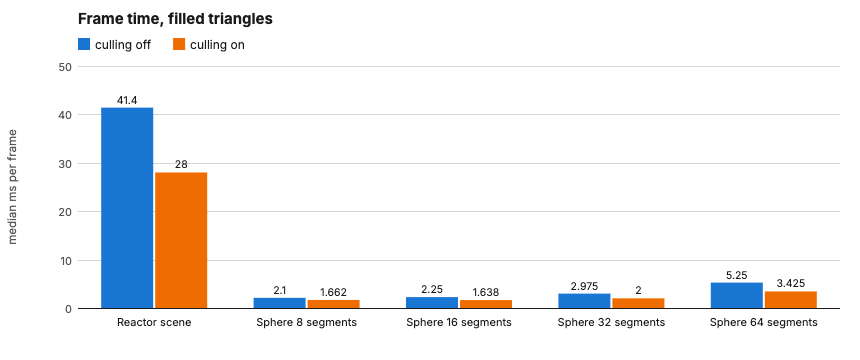
\includegraphics[width=0.48\linewidth]{figures/10-bench-chart-culling.png}\hfill
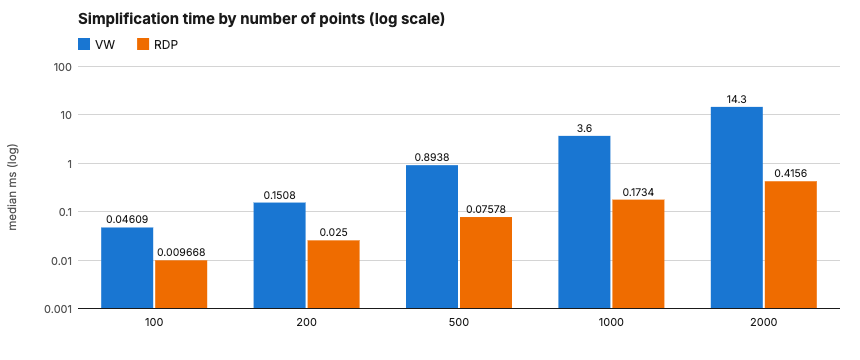
\includegraphics[width=0.48\linewidth]{figures/10-bench-chart-vw.png}
\caption{Charts saved from the Benchmark tab. Left: frame time with culling off and on. Right: time to simplify, VW against RDP.}
\label{fig:benchcharts}
\end{figure}

\chapter{LIMITATIONS, CONCLUSION AND FUTURE WORK}\nonum

\section{Limitations}
\begin{itemize}
\item \textbf{No clipping.} A triangle with a corner behind the camera is skipped completely, not cut. In the demo scene this skipped 359 of 15,412 triangles when culling was off.
\item \textbf{Flat shading.} Each triangle has one colour, so curved objects show their flat faces.
\item \textbf{One-sided planes.} A plane has one front side and disappears when seen from behind with culling on.
\item \textbf{Visvalingam--Whyatt is $O(n^2)$.} It is fine for the lab but would be slow for millions of points.
\item \textbf{One run, one machine.} The benchmark was run once in headless Chrome. The relative results are useful, but the exact milliseconds will differ on other computers.
\item \textbf{Bresenham is not faster in JavaScript,} as the benchmark shows.
\item \textbf{The interface has no automated tests.} We checked it by hand, in Chrome on macOS only.
\item \textbf{Lighting, fog and bloom} are simple extras and are not among the four required algorithms.
\end{itemize}

\section{Conclusion}
RenderLab has the four required algorithms (Bresenham, back-face culling, alpha compositing and Visvalingam--Whyatt) as plain TypeScript with no graphics library. Each has a lab that shows the formulas, the numbers at every step, and a comparison. Other labs cover transformations, determinants, quaternions, the outer product, the sine rule, line intersection, bases and handedness. All 487 tests pass, and all 195 controls passed our click-through after two layout fixes. The benchmark gave some results we did not expect: DDA was faster than Bresenham in JavaScript, and Visvalingam--Whyatt was about 34 times slower than RDP at 2,000 points.

\begin{table}[H]
\centering
\caption{Contribution of each student}
\label{tab:contrib}
\small
\begin{tabularx}{\linewidth}{@{}p{3.2cm}L@{}}
\toprule
Name & Work\\
\midrule
Yasharth Singh & TODO: fill in before submission\\
Rakshit Suneja & TODO: fill in before submission\\
\bottomrule
\end{tabularx}
\end{table}

\section{Future Work}
\begin{itemize}
\item Port the core to Rust and WebAssembly. Bresenham's whole-number arithmetic should then show the speed benefit that JavaScript does not give, and the benchmark can be repeated to check.
\item Use a heap in Visvalingam--Whyatt to make it $O(n\log n)$.
\item Cut triangles at the near plane (clipping) so they do not disappear close to the camera.
\item Add smooth shading and textures.
\item Add automated tests for the interface.
\end{itemize}


% ------------------------------------------------------------ REFERENCES
\cleardoublepage
\addtocontents{toc}{\protect\vspace{6pt}}
\addtocline{\bfseries}{References}
\renewcommand{\bibname}{REFERENCES}
\begin{singlespace}
\small
\bibliographystyle{IEEEtran}
\bibliography{references}
\end{singlespace}

\end{document}
